\chapter{Estimation}

\begin{definition}[Estimator]
    An \textbf{estimator} is a formula, that tells 
    how to calculate the value of an estimate based 
    on the observations contained in a sample.
\end{definition}

For example, the sample mean 
\[
    \ols{X} = \frac{X_1 + X_2 + \cdots + X_n}{n}
\]
is a rule that tells us how to calculate the estimate of the population mean $\mu$ based on the observations in a sample.

\begin{theorem}[Mean Squared Error]
    For an estimator $\hat{\mu}(X)$ of $\mu = \mu(\theta)$, the mean-squared error is 
    \begin{equation}
        MSE(\hat{\mu}) = Var[\hat{\mu}(X) \> | \> \theta] + \bias(\hat{\mu} \> | \> \theta)^2
    \end{equation}
    where $\bias (\hat{\mu} \> | \> \theta) = \mathbb{E}_\theta [\hat{\mu}(X) \> | \> \theta] - \mu$.
\end{theorem}
\begin{proof}
    Consider the following decision framework:
    \begin{itemize}
        \item $X \sim P_\theta,\> \theta \in \Theta$.
        \item The parameter of interest, $\mu(\theta)$ is a certain function.
        \item Action space, $\mathcal{A} = \{ \mu = \mu(\theta), \> \theta \in \Theta \}$.
        \item Decision procedure (or estimator), $\hat{\mu}(X) : \mathcal{X} \to \mathcal{A}$.
        \item Squared error loss as loss function: $L(\theta, a) = [a - \mu(\theta)]^2$.
    \end{itemize}
    with the setup above, the MSE is equal to the risk of decision,
    \begin{align*}
        R(\theta, \hat{\mu}(X)) &= \mathbb{E}[L(\left(\theta, \hat{\mu}(X) \right) \> | \> \theta]\\
        &= \mathbb{E}[\left(\hat{\mu}(X) - \mu(\theta) \right)^2 \> | \> \theta]\\
        &= \mathbb{E}[\left(\hat{\mu}(X) - \mu \right)^2 \> | \> \theta]\\
        &= Var[\hat{\mu}(X) \> | \> \theta] + 
            \big(\underbrace{\mathbb{E}[\hat{\mu}(X) \> | \> \theta] - \mu}_{\bias(\hat{\mu} | \theta)} \big)^2
    \end{align*}
\end{proof}

\section{Point Estimators}
A \textbf{point estimator} is a function of the sample data that provides a single value as an estimate of an unknown population parameter. Since the estimator is calculated from a random sample, it is itself a random variable and has a probability distribution, called the \textbf{sampling distribution}.

The sampling distribution of a point estimator describes how the estimator varies from sample to sample. Key properties of the sampling distribution include its mean (which relates to bias) and its variance (which relates to the precision of the estimator). Understanding the sampling distribution is fundamental for assessing the reliability of an estimator, constructing confidence intervals, and performing hypothesis tests.

% Table fits to paper width using tabularx
\begin{table}[h!]
\renewcommand{\arraystretch}{1.2}
\begin{tabularx}{\textwidth}{p{2.5cm}|l|l|X|l|X}
    & Target Parameter & Sample size & Point Estimator & $\mathbb{E}[\theta]$ & Standard Error \\
    \hline
    Population Mean & $\mu$ & $n$ & $\ols{X} = \frac{1}{n}\sum_{i=1}^n X_i$ & $\mu$ & $\frac{\sigma}{\sqrt{n}}$ \\
    Proportion & $p$ & $n$ & $\hat{p} = \frac{1}{n}\sum_{i=1}^n X_i$ & $p$ & $\sqrt{\frac{p(1-p)}{n}}$ \\
    Difference in Means & $\mu_1 - \mu_2$ & $m, n$ & $\ols{X} - \ols{Y}$ & $\mu_1 - \mu_2$ & $\sqrt{\frac{\sigma_1^2}{m} + \frac{\sigma_2^2}{n}}$ \\
    Difference in Proportions & $p_1 - p_2$ & $m, n$ & $\hat{p}_1 - \hat{p}_2$ & $p_1 - p_2$ & $\sqrt{\frac{p_1(1-p_1)}{m} + \frac{p_2(1-p_2)}{n}}$ \\
    \hline
\end{tabularx}
\end{table}

\begin{example}
     In a random sample of 80 components of a certain
 type, 12 are found to be defective.
 \begin{enumerate}
    \item Find a point estimate of the proportion of non-defective components.
    \item Find the standard error of the point estimate.
 \end{enumerate}
\end{example}
\begin{solution}
    \begin{enumerate}
        \item With $p$ as the proportion of non-defective components,
        the point estimate for proportion is
        \[
            \hat{p} = \frac{80-12}{80} = 0.85.
        \]
        
        \item The standard error of the point estimate of non-defective proportion is
        \[
            SE(\hat{p}) = \sqrt{\frac{\hat{p}(1-\hat{p})}{n}} = \sqrt{\frac{0.85 \times 0.15}{80}} \approx 0.0399.
        \]
    \end{enumerate}
\end{solution}

\begin{example}
    Let $X$ and $Y$ denote the strengths of concrete beam and cylinder specimens, respectively.
    The following data were obtained:

    \begin{table}[h!]
    \centering
    \small
    \begin{tabular}{l|ccccccc}
    \hline
    $X$ & 5.9 & 7.2 & 7.3 & 6.3 & 8.1 & 6.8 & 7.0 \\
        & 7.6 & 6.8 & 6.5 & 7.0 & 6.3 & 7.9 & 9.0 \\
        & 8.2 & 8.7 & 7.8 & 9.7 & 7.4 & 7.7 & 9.7 \\
        & 7.8 & 7.7 & 11.6 & 11.3 & 11.8 & 10.7 & \\
    \hline
    $Y$ & 6.1 & 5.8 & 7.8 & 7.1 & 7.2 & 9.2 & 6.6 \\
        & 8.3 & 7.0 & 8.3 & 7.8 & 8.1 & 7.4 & 8.5 \\
        & 8.9 & 9.8 & 9.7 & 14.1 & 12.6 & 11.2 & \\
    \hline
    \end{tabular}
    \end{table}
    Suppose $\mathbb{E}[X] = \mu_1$, $Var[X] = \sigma^2_1$, $\mathbb{E}[Y] = \mu_2$, and $Var[Y] = \sigma^2_2$.
    \begin{enumerate}
        \item Show that $\ols{X} - \ols{Y}$ is an unbiased estimator of $\mu_1 - \mu_2$.
        \item Find the mean and standard error of the point estimate of $\mu_1 - \mu_2$.
    \end{enumerate}
\end{example}
\begin{solution}
    \begin{enumerate}
        \item Since $X$ and $Y$ are independent, we have
        \[
            \mathbb{E}[\ols{X} - \ols{Y}] = \mathbb{E}[\ols{X}] - \mathbb{E}[\ols{Y}] = \mu_1 - \mu_2.
        \]
        Thus, $\ols{X} - \ols{Y}$ is an unbiased estimator of $\mu_1 - \mu_2$.
        
        \item The mean of the point estimate is 
        \[
            \mathbb{E}[\ols{X} - \ols{Y}] = \ols{x} - \ols{y} = 8.141 - 8.575 = 0.434.
        \]
        The variance of the difference in means is
        \[
            Var[\ols{X} - \ols{Y}] = Var[\ols{X}] + Var[\ols{Y}] = \frac{\sigma^2_1}{n} + \frac{\sigma^2_2}{m}.
        \]
        And 
        \[
            \sigma_{\ols{X} - \ols{Y}} = \sqrt{\frac{\sigma^2_1}{n} + \frac{\sigma^2_2}{m}}.
        \]
        Since $\sigma^2_1$ and $\sigma^2_2$ are unknown, we use $s^2_X$ and $s^2_Y$ to estimate $\sigma^2_1$ and $\sigma^2_2$ respectively. Thus,

        The standard error of the point estimate is
        \[
            S_{\ols{X} - \ols{Y}} = \sqrt{\frac{S^2_X}{n} + \frac{S^2_Y}{m}} = 
            \sqrt{\frac{1.666^2}{27} + \frac{2.104^2}{20}} = 0.5687.
        \]

    \begin{figure}[ht]
    \centering
    \makebox[\textwidth]{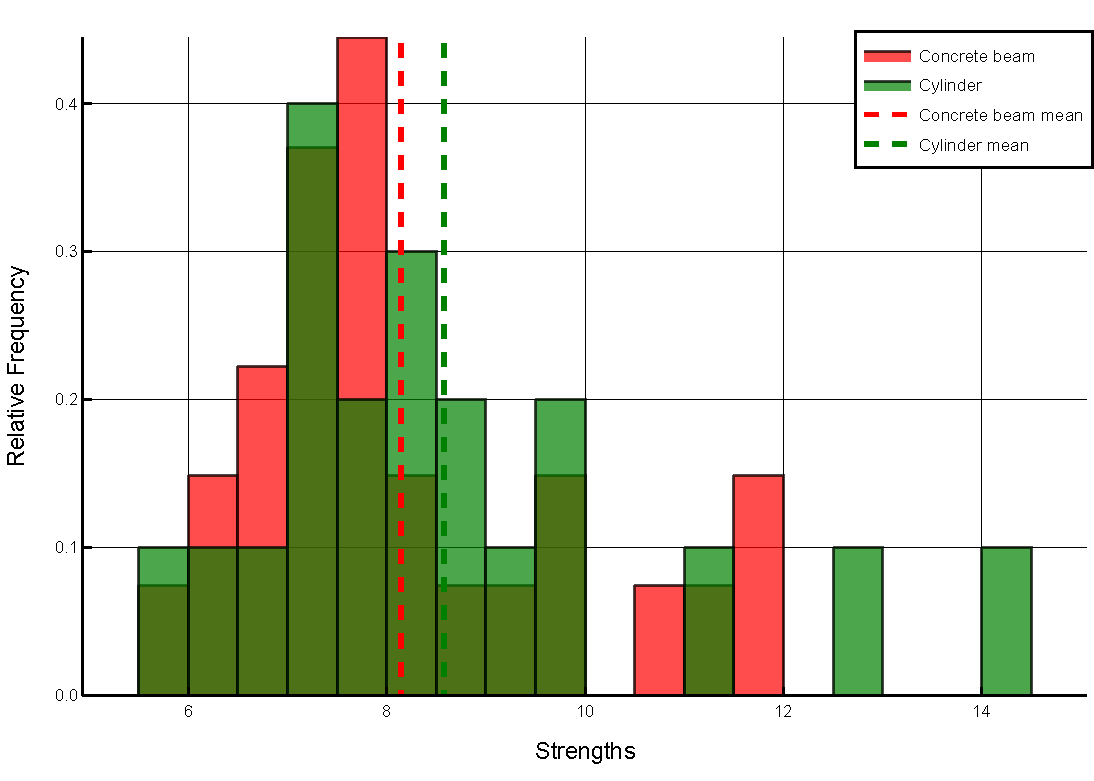
\includegraphics[width=0.8\paperwidth]{./images/hist01.pdf}}
    \end{figure}

    \end{enumerate}
\end{solution}
\begin{remark}
    Note that $S_1$ is not an unbiased estimator of $\sigma_1$. 
    Similarly, $S_1 / S_2$ is not an unbiased estimator of $\sigma_1 / \sigma_2$.
\end{remark}

\section{Evaluating the Estimators}

Suppose $\hat{\theta}_1$ and $\hat{\theta}_2$ are two estimators of $\theta$ that are both 
unbiased. Then, although the distribution of each estimator 
is centered at the true value of $\theta$, the spreads of the 
distributions about the true value may be different.

Among all estimators of $\theta$ that are unbiased, we will always 
choose the one that has minimum variance. WHY? 

The resulting $\hat{\theta}$ is called the \textbf{minimum variance unbiased 
estimator (MVUE)} of $\theta$.

\begin{definition}[Unbiased estimator]
    The estimator $\hat{\mu}$ is unbiased if $\bias(\hat{\mu} \> | \> \theta) = 0$
\end{definition}

\begin{example}
    Let $X_1, X_2, X_3$ be a random sample of size 3 from a population with pmf 
    \[
        f(x|\lambda) = \begin{cases}
            \mfrac{\lambda^x\, e^{-\lambda}}{x!} & x = 0, 1, 2, \ldots\\
            0 & \text{otherwise}
        \end{cases}
    \]
    where $\lambda > 0$ is a parameter. Are the following estimators of $\lambda$ unbiased?
    \[
        \hat{\lambda}_1 = \frac{1}{4}(X_1 + 2X_2 + X_3), \quad \hat{\lambda}_2 = \frac{1}{9}(4X_1 + 3X_2 + 2X_3) 
    \]
    Given, $\hat{\lambda}_1$ and $\hat{\lambda}_2$ which one is more efficient? 
    
    Hence, find an unbiased estimator of $\lambda$ that is more efficient than both $\hat{\lambda}_1$ and $\hat{\lambda}_2$.
\end{example}
\begin{solution}
    Given the observations $X_1, X_2, X_3$ are i.i.d with $X_i \sim Poisson(\lambda)$, we have
    \[
        \mathbb{E}[X_i] = Var[X_i] = \lambda \quad \forall i = 1,2,3.
    \]
    It is easy to see that 
    \begin{align*}
        \mathbb{E}[\hat{\lambda}_1] &= \frac{1}{4}(\mathbb{E}[X_1] + 2\mathbb{E}[X_2] + \mathbb{E}[X_3]) = \frac{1}{4}(\lambda + 2\lambda + \lambda) = \lambda,\\
        \mathbb{E}[\hat{\lambda}_2] &= \frac{1}{9}(4\mathbb{E}[X_1] + 3\mathbb{E}[X_2] + 2\mathbb{E}[X_3]) = \frac{1}{9}(4\lambda + 3\lambda + 2\lambda) = \lambda.
    \end{align*}
    Thus, both $\hat{\lambda}_1$ and $\hat{\lambda}_2$ are unbiased estimators of $\lambda$.
    Next, we compute the variances of both estimators,
    \begin{align*}
        Var[\hat{\lambda}_1] &= \frac{1}{16}(Var[X_1] + 4Var[X_2] + Var[X_3]) = \frac{1}{16}(\lambda + 4\lambda + \lambda) = \frac{3\lambda}{8},\\
        Var[\hat{\lambda}_2] &= \frac{1}{81}(16Var[X_1] + 9Var[X_2] + 4Var[X_3]) = \frac{1}{81}(16\lambda + 9\lambda + 4\lambda) = \frac{29\lambda}{81}.
    \end{align*}
    By inspection, since $\frac{3}{8} = 0.375 > \frac{29}{81} \approx 0.358$, the estimator $\hat{\lambda}_2$ is more efficient than $\hat{\lambda}_1$.
    We have seen in previous section that the sample mean is always an unbiased estimator of the population mean irrespective of the population distribution. 
    The variance of the sample mean is always equal to $\frac{\sigma^2}{n}$, where $\sigma^2$ is the population variance and $n$ is the sample size. Thus 
    \[
        Var[\ols{X}] = \frac{Var[X_i]}{3} = \frac{1}{3}\lambda.
    \]
    The sample mean has even smaller variance than both $\hat{\lambda}_1$ and $\hat{\lambda}_2$. Thus, $\ols{X} = \mfrac{1}{3}\lambda$ is an unbiased estimator of $\lambda$ that is more efficient than both $\hat{\lambda}_1$ and $\hat{\lambda}_2$.
\end{solution}

\begin{example}
    Let $\hat{\theta}_1$ and $\hat{\theta}_2$ be unbiased estimators of $\theta$. Suppose $Var\left(\hat{\theta}_1\right) = 1$, $Var\left(\hat{\theta}_2\right) = 2$ and $\cov \left(\hat{\theta}_1, \hat{\theta}_2\right) = \frac{1}{2}$. What are the values of $c_1$ and $c_2$ for which $c_1\hat{\theta}_1 + c_2\hat{\theta}_2$ is an unbiased estimator of $\theta$ with minimum variance among unbiased estimators of this type?
\end{example}
\begin{solution}
    We want to find $c_1$ and $c_2$ such that $c_1\hat{\theta}_1 + c_2\hat{\theta}_2$ to be a minimum variance unbiased estimator of $\theta$. Then
    \begin{align*}
        \mathbb{E}[c_1\hat{\theta}_1 + c_2\hat{\theta}_2] = \theta &\implies c_1\mathbb{E}[\hat{\theta}_1] + c_2\mathbb{E}[\hat{\theta}_2] = \theta\\
        &\implies c_1\theta + c_2\theta = \theta\\
        &\implies c_1 + c_2 = 1\\
        &\implies c_2 = 1 - c_1.
    \end{align*}
    Therefore,
    \begin{align*}
        Var[c_1\hat{\theta}_1 + c_2\hat{\theta}_2] &= c_1^2 Var[\hat{\theta}_1] + c_2^2 Var[\hat{\theta}_2] + 2c_1c_2 \cov[\hat{\theta}_1, \hat{\theta}_2]\\
        &= c_1^2 (1) + 2(1 - c_1)^2 + 2c_1(1 - c_1)\left(\frac{1}{2}\right)\\
        &= 3c_1^2 - 3c_1 + 2.
    \end{align*}
    To find the minimum variance, we differentiate $Var[c_1\hat{\theta}_1 + c_2\hat{\theta}_2]$ with respect to $c_1$ and set it to zero, that is
    \[
        \frac{\mathrm{d}}{\mathrm{d}c_1}Var[c_1\hat{\theta}_1 + c_2\hat{\theta}_2] = 6c_1 - 3 = 0 \quad \implies c_1 = \frac{1}{2}.
    \]
    Thus, $c_2 = 1 - c_1 = \mfrac{1}{2}$. Therefore, the minimum variance unbiased estimator of $\theta$ is 
    \[
        \hat{\theta} = \frac{1}{2}\hat{\theta}_1 + \frac{1}{2}\hat{\theta}_2.
    \]
    In fact, if $\theta_1$ and $\theta_2$ are both unbiased estimators of $\theta$, then the 
    linear combination $c_1\theta_1 + c_2\theta_2$ is also an unbiased estimator of $\theta$ for any $c_1, c_2$ such that $c_1 + c_2 = 1$.
    Hence
    \[
        \mathcal{C} = \{ \hat{\theta} = c\hat{\theta}_1 + (1-c)\hat{\theta}_2 \> | \> c \in \mathbb{R} \}
    \]
\end{solution}

\textbf{Rule of thumb choosing a good estimator}:
\begin{itemize}
    \item Unbiasedness: $\mathbb{E}[\hat{\theta}] = \theta$.
    \item Minimum variance: A good estimator should has smaller $Var[\hat{\theta}]$, the smaller the better.
\end{itemize}

\subsection{Method of Moments (MoM) Estimator}

The method of moments is a technique for estimating population parameters by equating sample moments to theoretical moments. Moments are quantitative measures related to the shape of a distribution, such as the mean (first moment), variance (second moment), skewness (third moment), and kurtosis (fourth moment).
The method of moments involves the following steps:

\begin{enumerate}
    \item Calculate the theoretical (population) moments as functions of the unknown parameters.
    \item Calculate the corresponding sample moments from the observed data.
    \item Set the population moments equal to the sample moments to create a system of equations.
    \item Solve the system of equations for the unknown parameters to obtain the MoM estimators.
\end{enumerate}

\begin{example}
    Let $X_1, X_2, \ldots, X_n$ be a random sample from a population with pdf 
    \[
        f(x|\theta) = \begin{cases}
            \theta x^{\theta - 1} & 0 < x < 1\\
            0 & \text{otherwise}
        \end{cases}
    \]
    where $\theta > 0$ is an unknown parameter. Find the method of moments estimator of $\theta$.
\end{example}
\begin{solution}
    To find the method of moments estimator, we shall equate the first population moment to the sample moment.
    The first population moment $\mathbb{E}[X]$ is given by
    \begin{align*}
        \mathbb{E}[X] &= \int_0^1 x f(x|\theta) \> \mathrm{d}x\\
        &= \int_0^1 x (\theta x^{\theta - 1} )\> \mathrm{d}x\\
        &= \theta \int_0^1 x^{\theta} \> \mathrm{d}x\\
        &= \theta \left[ \frac{x^{\theta + 1}}{\theta + 1} \right]_{x=0}^{x=1} = \frac{\theta}{\theta + 1} = M_X(x).
    \end{align*}
    We know that the first moment $M_X(x) = \ols{X}$. Now setting $M_X(x) = \mathbb{E}{X}$ 
    and solving for $\theta$, we have
    \[
        \ols{X} = \frac{\theta}{\theta + 1} 
    \]
    that is
    \[
        \theta = \frac{\ols{X}}{1 - \ols{X}}.
    \]
    where $\ols{X} = \mfrac{1}{n}\sum_{i=1}^n X_i$ is the sample mean. Thus, the statistic 
    $\mfrac{\ols{X}}{1 - \ols{X}}$ is an estimator of parameter $\theta$. We write 
    \[
        \hat{\theta} = \frac{\ols{X}}{1 - \ols{X}}.
    \]
    Now let say we have the following sample data:
    \[
        0.44,\quad 0.55,\quad 0.60,\quad 0.30
    \]
    we have $\ols{X} = \mfrac{0.44 + 0.55 + 0.60 + 0.30}{4} = 0.4725$, and the estimate of $\theta$ is
    \[
        \hat{\theta} = \frac{0.4725}{1 - 0.4725} = 0.8957.
    \]
\end{solution}

\begin{example}
    Let $X \sim \mathcal{N}(\mu, \sigma^2)$, and $X_1, X_2, \ldots X_n$ be a random sample of size $n$ from $X$. 
    Find the method of moments estimators of $\mu$ and $\sigma^2$.
\end{example}
\begin{solution}
    The first population moment is 
    \[
        \mathbb{E}[X] = \mu.
    \]
    The second population moment is 
    \[
        \mathbb{E}[X^2] = Var[X] + (\mathbb{E}[X])^2 = \sigma^2 + \mu^2.
    \]
    The first sample moment is 
    \[
        M_1 = \ols{X} = \frac{1}{n}\sum_{i=1}^n X_i.
    \]
    The estimator of the parameter $\mu$ is $\hat{\mu} = \ols{X}$, that is
    \[
        \hat{\mu} = \ols{X} = \frac{1}{n}\sum_{i=0}^{n} X_i.
    \]
    
    Next, we equate the second population moment to the second sample moment. Note that the variance of the population is
    \begin{align*}
        \sigma^2 &= \mathbb{E}[X^2] - \mu^2\\
        &= M_2 - \mu^2\\
        &= \frac{1}{n}\sum_{i=1}^{n}X^2_i - (\ols{X})^2.\\
        &= \frac{1}{n} \sum_{i=1}^{n}(X_i - \ols{X})^2.
    \end{align*}
    The last line follows from the fact that
    \begin{align*}
        \frac{1}{n} \sum_{i=1}^{n}(X_i - \ols{X})^2 &= \frac{1}{n}\sum_{i=1}^{n}(X_i^2 - 2X_i\ols{X} + (\ols{X})^2)\\
        &= \frac{1}{n}\sum_{i=1}^{n}X_i^2 - 2\ols{X}\frac{1}{n}\sum_{i=1}^{n}X_i + \frac{1}{n}\sum_{i=1}^{n}(\ols{X})^2\\
        &= \frac{1}{n}\sum_{i=1}^{n}X_i^2 - 2\ols{X}(\ols{X}) + \ols{X}^2\\
        &= \frac{1}{n}\sum_{i=1}^{n}X_i^2 - \ols{X}^2.
    \end{align*}
    Thus, the estimator of the parameter $\sigma^2$ is 
    \[
        \hat{\sigma}^2 = \frac{1}{n} \sum_{i=1}^{n}(X_i - \ols{X})^2.
    \]
\end{solution}

\begin{theorem}
    Let $X_1, X_2, \ldots, X_n$ be a random sample with $\mathbb{E}[X_i] = \mu$ 
    and $Var[X_i] = \sigma^2$. Then 
    \[
        \tilde{S}^2 = \frac{1}{n}\sum_{i=1}^{n}(X_i - \ols{X})^2 
    \]
    is a \textit{biased estimator} of $\sigma^2$ but that 
    \[
        S^2 = \frac{1}{n-1}\sum_{i=1}^{n}(X_i - \ols{X})^2
    \]
    is an \textit{unbiased estimator} of $\sigma^2$.
\end{theorem}
\begin{proof}
    From previous example, we can see that 
    \begin{equation*}
    \begin{tikzpicture}[remember picture, overlay, baseline=(eq.base)]
        \node[anchor=base west] (eq) at (0,0) {$
            \displaystyle \sum_{i=1}^{n} (X_i - \ols{X})^2 = \sum_{i=1}^{n} X_i^2 - n(\ols{X})^2 \tag{{\color{red} $\bigstar$}}
        $};
        \node[anchor=base west, right=5.5cm of eq] (tag) {};
    \draw[red, thick, dashed] (tag.west) -- (eq.east);
    \end{tikzpicture}
    \hspace{7.7cm} \label{eq:es1.0}
    \end{equation*}

    Hence, we use this and the fact that 
    \[
        \mathbb{E}[X_i^2] = Var[X_i] + (\mathbb{E}[X_i])^2 = \sigma^2 + \mu^2,
    \]
    and
    \[
        \mathbb{E}[\ols{X}^2] = Var[\ols{X}] + (\mathbb{E}[\ols{X}])^2 = \frac{\sigma^2}{n} + \mu^2,
    \]
    and 
    take expectation on both sides of \eqref{eq:es1.0}, we have
    \begin{align*}
        \mathbb{E}\left[\sum_{i=1}^{n} (X_i - \ols{X})^2\right] &= \mathbb{E}\left[\sum_{i=1}^{n} X_i^2 - n(\ols{X})^2\right]\\
        &= \sum_{i=1}^{n} \mathbb{E}[X_i^2] - n\mathbb{E}[(\ols{X})^2]\\
        &= n(\sigma^2 + \mu^2) - n\left(\frac{\sigma^2}{n} + \mu^2\right)\\
        &= (n-1)\sigma^2.
    \end{align*}
    It follows that 
    \[
        \mathbb{E}[\tilde{S}^2] = \frac{1}{n} \mathbb{E}\left[\sum_{i=1}^{n}(X_i - \ols{X})^2\right] = \frac{n-1}{n}\sigma^2 \neq \sigma^2,
    \]
    and that $\tilde{S}^2$ is biased since $\mathbb{E}[\tilde{S}^2] \neq \sigma^2$.
    However,
    \[
        \mathbb{E}[S^2] = \frac{1}{n-1} \mathbb{E}\left[\sum_{i=1}^{n}(X_i - \ols{X})^2\right] = \sigma^2,
    \]
    thus we can see that $S^2$ is an unbiased estimator of $\sigma^2$.
\end{proof}

\section{Maximum Likelihood Estimator (MLE)}

The maximum likelihood estimation (MLE) is a method used to estimate the parameters of a statistical model. The MLE is the parameter value that maximizes the likelihood function, which measures how likely it is to observe the given sample data for different parameter values.
Next, we describe this method in detail.

\begin{definition}[Likelihood function and MLE]
    Let $X_1, X_2, \ldots, X_n$ be a random sample from a population with pdf/pmf $f(x|\theta)$, where $\theta \in \Theta$ is an unknown parameter. The likelihood function is defined as
    \[
        L(\theta|x) = \prod_{i=1}^{n} f(x_i | \theta).
    \]
    The maximum likelihood estimator (MLE) of $\theta$ is the value of $\theta$ that maximizes the likelihood function $L(\theta)$.
\end{definition}

This definition state that the likelihood function $L(\theta | x)$ is the product of the individual pdf evaluated at each observation in the sample, given the parameter $\theta$. 
The likelihood function represents the joint density of a random sample $X_1, X_2, \ldots, X_n$ given the parameter $\theta$.
The MLE is the value of $\theta$ that makes the observed data most probable.

The $\theta$ that maximizes $L(\theta|x)$ is called the maximum likelihood estimate and is denoted by $\hat{\theta}$.
\[
    \hat{\theta} = \arg\max_{\theta \in \Theta} L(\theta | x).
\]

In practice, it is often more convenient to work with the natural logarithm of the likelihood function, known as the log-likelihood function:
\[
    \ell(\theta) = \ln L(\theta) = \sum_{i=1}^{n} \ln f(x_i | \theta).
\]
Maximizing the log-likelihood function is equivalent to maximizing the likelihood function itself, as the logarithm is a monotonically increasing function.

\begin{example}
    Let $X \sim B(1,p)$, a Bernoulli random variable with parameter $p$, with pmf 
    \[
        f(x|p) = \mathbb{P}[X = x | p] = \begin{cases}
            p^x (1-p)^{1-x} & x = 0, 1\\
            0 & \text{otherwise}
        \end{cases}
    \]
    where $0 < p < 1$. Let $X_1, X_2, \ldots, X_n$ be a random sample of size $n$ from $X$. Find the maximum likelihood estimator of $p$.
\end{example}
\begin{solution}
    Our goal is to find the value of $p$ that maximizes the likelihood function based on the observed sample data 
    $X = (X_1, X_2, \ldots, X_n)$. Note that $X_1, X_2, \ldots, X_n$ are i.i.d. Thus, the likelihood function is given by
    \begin{align*}
        L(p|x) &= \prod_{i=1}^{n} f(x_i | p)\\
        &= \prod_{i=1}^{n} p^{x_i} (1-p)^{1-x_i}\\
        &= p^{\sum_{i=1}^{n} x_i} (1-p)^{\sum_{i=1}^{n}(1-x_i)}\\
        &= p^{\sum_{i=1}^{n} x_i} (1-p)^{n - \sum_{i=1}^{n} x_i}.
    \end{align*}
    We can simplify the notation by letting $S_n = \sum_{i=1}^{n} x_i$. We want to choose $p$ such that $L(p|x)$ is maximized. Take the logarithm of the likelihood function, we have
    \[
        \ell(p|x) = \ln L(p|x) = S_n \ln p + (n - S_n) \ln(1-p).
    \]
    To find the maximum, we take the derivative of $\ell(p|x)$ with respect to $p$ and set it to zero:
    \begin{align*}
        \frac{\partial \ell(p|x)}{\partial p} &= \frac{S_n}{p} - \frac{n - S_n}{1-p} = 0\\
        \Rightarrow S_n(1-p) &= (n - S_n)p\\
        \Rightarrow S_n - S_n p &= np - S_n p\\
        \Rightarrow S_n &= np\\
        \Rightarrow \hat{p} &= \frac{S_n}{n} = \frac{1}{n}\sum_{i=1}^{n} x_i = \ols{X}.
    \end{align*}
    The sample mean (proportion) $\ols{X}$ is the maximum likelihood estimator of $p$.
\end{solution}

\subsection{MLE based on grouped data}

In some cases, data may be grouped into intervals or categories, and we may not have access to the individual data points. In such situations, we can still use the maximum likelihood estimation (MLE) method to estimate parameters based on the grouped data.

In the complete data case, the likelihood is measured by the density (or probability) $f(x_i)$ at the known data point $x_i$. The likelihood function is the product of those densities for the points in the sample. In the interval grouped data case, we measure likelihood of a point as the probability of the interval in which that point occurs. For a data point in the interval $(c_{j-1}, c_j]$, the probability of that interval is $[F(c_j; \theta) - F(c_{j-1}; \theta)]$. The likelihood function is the product of those interval probabilities for all of the sample points. Since there are $n_j$ sample points in the interval $(c_{j-1}, c_j]$, the likelihood function will include a factor of $[F(c_j; \theta) - F(c_{j-1}; \theta)]^{n_j}$ for those $n_j$ points. The overall likelihood function is the product of all of those factors:

\begin{definition}[MLE based on grouped data]
    If the data is grouped into $k$ intervals with counts $n_1, n_2, \ldots, n_k$ in each interval, the likelihood function for the grouped data is given by
    \[
        L(\theta|x) = \prod_{j=1}^{k} [F(c_j|\theta) - F(c_{j-1}|\theta)]^{n_j},
    \]
    where $F(x|\theta)$ is the cumulative distribution function (CDF) of the underlying distribution, and $[c_{j-1}, c_j)$ is the $j$-th interval.
\end{definition}

\begin{example}
    For a group of insurance policies, you are given:
    \begin{enumerate}
        \item The losses follow the distribution function
        \[
            F(x|\theta) = 1 - \frac{\theta}{x}, \quad \theta < x < \infty.
        \]
        \item A sample of 20 losses is grouped as follows:
        \begin{table}[h!]
        \centering
        \begin{tabular}{|c|c|}
        \hline
        Interval & Number of loss \\
        \hline
        $x \leq 10$ & 9 \\
        $10 < x \leq 25$ & 6\\
        $x > 25$ & 5\\
        \hline
        \end{tabular}
        \end{table}
    \end{enumerate}
    Calculate the maximum likelihood estimate of $\theta$.
\end{example}
\begin{solution}
    The likelihood function is the product of the probabilities of observing the data in each interval, 
    The probability for the interval $x \leq 10$ is given by 
    \[ 
        F(10|\theta) = 1 - \frac{\theta}{10},
    \]
    the probability for the interval $10 < x \leq 25$ is given by 
    \[
        F(25|\theta) - F(10|\theta) = \left(1 - \frac{\theta}{25}\right) - \left(1 - \frac{\theta}{10}\right) = \frac{\theta}{10} - \frac{\theta}{25} = \frac{3}{50}\theta,    
    \] 
    and the probability for the interval $x > 25$ is given by 
    \[
        1 - F(25|\theta) = 1 - \left(1 - \frac{\theta}{25}\right) = \frac{\theta}{25}.
    \]
    Then, the likelihood function is given by 
    \begin{align*}
        L(\theta) &= [F(10|\theta)]^{n_1} [F(25|\theta) - F(10|\theta)]^{n_2} [1 - F(25|\theta)]^{n_3}\\
        &= \left(1 - \frac{\theta}{10}\right)^{9} \left(\frac{3\theta}{50}\right)^{6} \left(\frac{\theta}{25}\right)^{5}\\
        &= c(10 - \theta)^9 \theta^{11},
    \end{align*}
    where $c = \mfrac{3^6}{50^6 \times 25^5}$ is a constant. To find the value of $\theta$ that maximizes $L(\theta)$, we take the logarithm of the likelihood function:
    \[
        \ell(\theta) = \ln L(\theta) = \ln c + 9 \ln(10 - \theta) + 11 \ln \theta.
    \]
    Next, we differentiate $\ell(\theta)$ with respect to $\theta$ and set it to zero:
    \begin{align*}
        \frac{\mathrm{d}\ell(\theta)}{\mathrm{d}\theta} &= \frac{9}{10 - \theta}(-1) + \frac{11}{\theta} = 0\\
        \Rightarrow -\frac{9}{10 - \theta} + \frac{11}{\theta} &= 0\\
        \Rightarrow 11(10 - \theta) &= 9\theta\\
        \Rightarrow 110 - 11\theta &= 9\theta\\
        \Rightarrow 110 &= 20\theta\\
        \Rightarrow \hat{\theta} &= 5.5
    \end{align*}
    Thus, the maximum likelihood estimate of $\theta$ is $\hat{\theta} = 5.5$.
\end{solution}

\begin{example}
    A grouped data set has 20 data points grouped into the following intervals:
    \begin{table}[h!]
    \centering
    \begin{tabular}{|c|c|c|c|c|}
    \hline
    Interval & $0 < x \leq 5$ & $5 < x \leq 10$ & $10 < x \leq 25$ & $x > 25$ \\
    \hline
    Number of data points & 4 & 7 & 6 & 3 \\
    \hline
    \end{tabular}
    \end{table}

    \begin{figure}[ht]
    \centering
    \makebox[\textwidth]{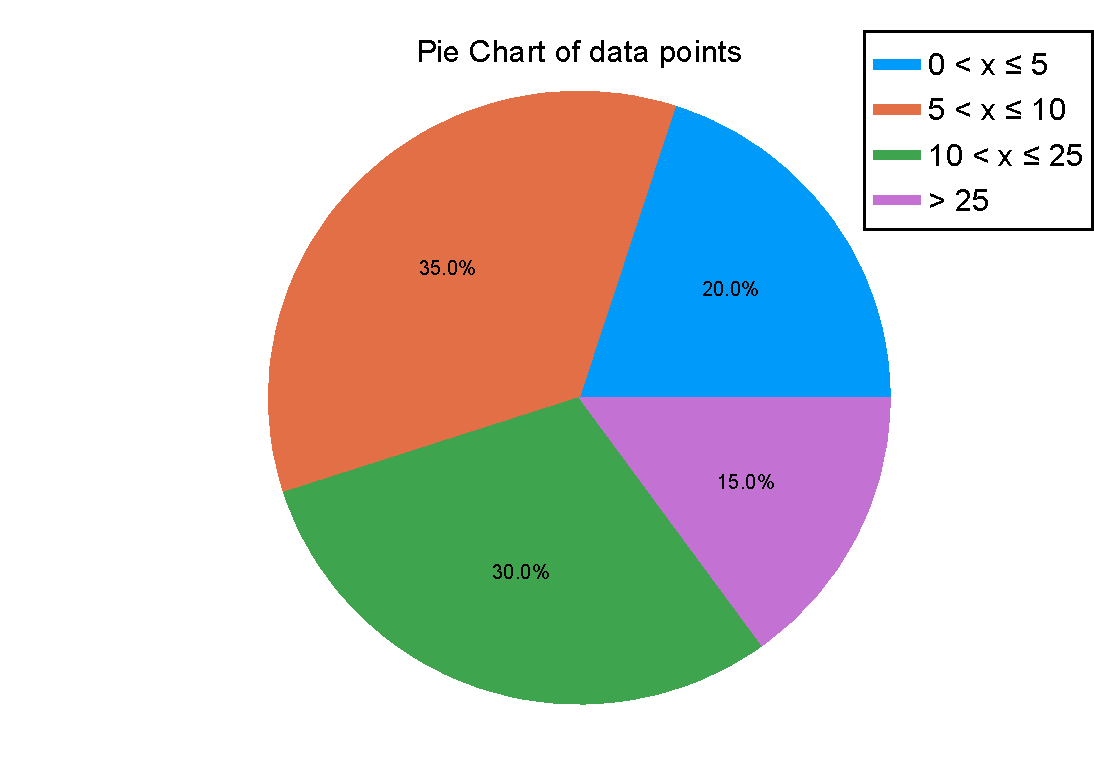
\includegraphics[scale=0.6]{./images/pie_chart.pdf}}
    \end{figure}
    
    Apply the maximum likelihood method to estimate the parameter $\theta$ of the following two cases:
    
    \begin{enumerate}
        \item The data follow the exponential distribution with parameter $\theta$,
        \item The data follow the uniform distribution on the interval $(0, \theta)$.
    \end{enumerate}
\end{example}
\begin{solution}
    \begin{enumerate}
        \item If we assume that the data follow the exponential distribution with parameter $\theta$, then the cdf is given by
        \[
            F(x|\theta) = 1 - e^{-\theta x}, \quad x > 0, \theta > 0.
        \]
        The likelihood function is given by
        \begin{align*}
            L(\theta) &= [F(5|\theta)]^{n_1} [F(10|\theta) - F(5|\theta)]^{n_2} [F(25|\theta) - F(10|\theta)]^{n_3} [1 - F(25|\theta)]^{n_4}\\
            &= (1 - e^{-5\theta})^4 (e^{-5\theta} - e^{-10\theta})^7 (e^{-10\theta} - e^{-25\theta})^6 (e^{-25\theta})^3\\
            &= c (1 - e^{-5\theta})^4 (e^{-5\theta})^7 (1 - e^{-5\theta})^6 (e^{-25\theta})^3\\
            &= c (1 - e^{-5\theta})^{10} (e^{-5\theta})^{10} (e^{-25\theta})^3\\
            &= c (1 - e^{-5\theta})^{10} e^{-50\theta},
        \end{align*}
        where $c = 1$ is a constant. To find the value of $\theta$ that maximizes $L(\theta)$, we take the logarithm of the likelihood function:
    
        \item In another case, if we assume that the data follow the uniform distribution on the interval $(0, \theta)$, then the cdf is given by
        \[
            F(x|\theta) = \begin{cases}
                \frac{x}{\theta} & 0 < x < \theta\\
                0 & \text{otherwise}
            \end{cases}
        \]
        The likelihood function is given by
        \begin{align*}
            L(\theta) &= [F(5|\theta)]^{n_1} [F(10|\theta) - F(5|\theta)]^{n_2} [F(25|\theta) - F(10|\theta)]^{n_3} [1 - F(25|\theta)]^{n_4}\\
            &= \left(\frac{5}{\theta}\right)^4 \left(\frac{10}{\theta} - \frac {5}{\theta}\right)^7 \left(\frac{25}{\theta} - \frac{10}{\theta}\right)^6 \left(1 - \frac{25}{\theta}\right)^3\\
            &= c \theta^{-20} (\theta - 25)^3,
        \end{align*}
        where $c = 5^4 \times 5^7 \times 15^6$ is a constant. To find the value of $\theta$ that maximizes $L(\theta)$, we take the logarithm of the likelihood function:
        \[
            \ell(\theta) = \ln L(\theta) = \ln c - 20 \ln \theta + 3 \ln(\theta - 25).
        \]
        Next, we differentiate $\ell(\theta)$ with respect to $\theta$ and set it to zero:
        \begin{align*}
            \frac{\mathrm{d}\ell(\theta)}{\mathrm{d}\theta} &= -\frac{20}{\theta} + \frac{3}{\theta - 25} = 0\\
            \Rightarrow -20(\theta - 25) + 3\theta &= 0\\
            \Rightarrow -20\theta + 500 + 3\theta &= 0\\
            \Rightarrow -17\theta + 500 &= 0\\
            \Rightarrow \hat{\theta} &= \frac{500}{17} \approx 29.41.
        \end{align*}
        Thus, the maximum likelihood estimate of $\theta$ is $\hat{\theta} = \frac{500}{17} \approx 29.41$. 
    \end{enumerate}
\end{solution}

\section*{Tutorials}

\begin{mdframed}
    \vspace{-0.25cm}
    \hspace{-0.25cm}
    \begin{Exercise}
        Given 20 observations on breakdown voltage for some materials
        \begin{center}
            \begin{tabular}{cccccccccc}
            24.46 & 25.61 & 26.25 & 26.42 & 26.66 & 27.15 & 27.31 & 27.54 & 27.74 & 27.94\\
            27.98 & 28.04 & 28.28 & 28.49 & 28.50 & 28.87 & 29.11 & 29.13 & 29.50 & 30.88\\
            \end{tabular}
        \end{center}

        Assume that after looking at the histogram, we think that 
the distribution of breakdown voltage is normal with 
mean value $\mu$.  What are some point estimators for $\mu$?
    \end{Exercise}

    \vspace{0.752cm}
    \begin{Exercise}
        The probability density function of the random variable $X$ is defined by 
        \[
            f(x|\lambda) = 1 - \frac{2}{3}\lambda + \lambda \sqrt{x}, \quad 0 \leq x \leq 1,
        \]
        and zero otherwise. What is the maximum likelihood estimate of the parameter $\lambda$ based on the 
        two independent observations $x_1 = \mfrac{1}{4}$ and $x_2 = \mfrac{9}{16}$?
    \end{Exercise}

    \vspace{0.752cm}
    \begin{Exercise}
        Consider that $X_1, X_2, \ldots, X_n$ is a random sample from a distribution with density 
        function
        \[
            f(x|\beta) = \begin{cases}
                \mfrac{x^6 e^{-x/\beta}}{\Gamma(7)\, \beta^7} & \text{if } x > 0\\
                0 & \text{otherwise}.
            \end{cases}
        \]
        What is the maximum likelihood estimate of $\beta$?
    \end{Exercise}

    \vspace{0.752cm}
    \begin{Exercise}
        Let $X_1, X_2, \ldots, X_n$ be a random sample from the uniform density 
        function
        \[
            f(x|\theta) = \begin{cases}
                \frac{1}{\theta} & \text{if } 2\theta \leq x \leq 3\theta\\
                0 & \text{otherwise}
            \end{cases}
        \]
        where $\theta > 0$. Show that the maximum likelihood estimate of $\theta$ is 
        \[
            \frac{1}{3}\, \max \{ X_1, X_2,\ldots ,X_n\}.
        \]
    \end{Exercise}

    \begin{Exercise}
        What is the maximum likelihood estimate of $\beta$ if five values 
        $\mfrac{4}{5}, \mfrac{2}{3}, 1, \mfrac{3}{2}, \mfrac{5}{4}$ were drawn from the 
        population for which
        $\displaystyle f(x|\beta) = \frac{1}{2}(1 + \beta)^5 \left(\frac{x}{2}\right)^\beta$?
    \end{Exercise}

    \begin{Exercise}
        Eight independent trials are conducted of a given system with the following results: 
        \[S, F, S, F, S, S, S, S\] 
    where $S$ denotes the success and $F$ denotes
    the failure. What is the maximum likelihood estimate of the probability of
    successful operation $p$?
    \end{Exercise}

    \begin{Exercise}
    Suppose fertilizer-1 has a mean yield per acre of $\mu_1$
    with variance $\sigma^2$, whereas the expected yield for fertilizer-2 is $\mu_2$ with the
    same variance $\sigma^2$. Let $S^2_i$ denote the sample variances of yields based on
    sample sizes $n_1$ and $n_2$ respectively, of the two fertilizers.
    \begin{enumerate}
        \item Show that the pooled (combined) estimator 
        \[
            \hat{\sigma}^2 = \frac{(n_1 - 1)S^2_1 + (n_2 - 1)S^2_2}{n_1 + n_2 - 2}
        \]
        is an unbiased estimator of $\sigma^2$.
        \item The measurements for the two types of fertilizers were obtained independently, with 
        testing samples of $n_1 = n_2 = 100$, the following sample means and variances were computed:
        \[
            \ols{x}_1 = 179.3 \text{ yield per acre}, \quad \ols{x}_2 = 190.0 \text{ yield per acre},
        \]
        \[
            s^2_1 = 1440.80, \quad s^2_2 = 1960,
        \]
        Estimate the difference mean yied per acre, and the pooled variance of two fertilizers.
    \end{enumerate}
    \end{Exercise}

    \vspace{0.752cm}
    \begin{Exercise}
        A random sample $X_1, X_2, \ldots, X_n$ of size $n$ is selected from a normal distribution 
        with variance $\sigma^2$. Let $S^2$ be the unbiased estimator of $\sigma^2$, and 
        $T$ be the maximum likelihood estimator of $\sigma^2$. If $20T - 19S^2 = 0$, then what is 
        the sample size?
    \end{Exercise}

    \begin{Exercise}
        A box contains 50 red and blue balls out of which are red. A sample
 of 30 balls is to be selected without replacement. If $X$ denotes the number
 of red balls in the sample, then find an estimator for using the \textit{moment
 method}.
    \end{Exercise}

    \begin{Exercise}
        You are given:
        \begin{enumerate}
            \item Losses follow an exponential distribution with mean $\theta$.
            \item A random sample of 20 losses is observed as follows:
            \begin{center}
                \begin{tabular}{|c|c|}
                    \hline
                    Loss Range & Frequency\\
                    \hline
                    $[0,1000]$ & $7$\\
                    $(1000, 2000]$ & $6$\\
                    $(2000, \infty)$ & $7$\\
                    \hline
                \end{tabular}
            \end{center}
        \end{enumerate}
        Calculate the maximum likelihood estimate of $\theta$.
    \end{Exercise}
\end{mdframed}